\documentclass{article}

% Language setting
% Replace `english' with e.g. `spanish' to change the document language
\usepackage[english]{babel}
\usepackage{float}
\usepackage{array}
% Set page size and margins
% Replace `letterpaper' with `a4paper' for UK/EU standard size
\usepackage[letterpaper,top=1cm,bottom=2cm,left=2cm,right=2cm,marginparwidth=1.75cm]{geometry}

\usepackage{longtable} 
\usepackage{multicol}
\usepackage[dvipsnames]{xcolor}
% Useful packages 
\usepackage{bbding}
\usepackage{pifont}
\usepackage{wasysym}

\usepackage{mathtools}
\usepackage{multirow}
\usepackage{amsmath}
\usepackage{graphicx}
\usepackage[colorlinks=true, allcolors=blue]{hyperref}
\usepackage{makeidx}
\setlength{\columnsep}{1cm}
\usepackage{xcolor}
\usepackage{graphicx}
\usepackage{tcolorbox}
\usepackage{algpseudocode} 
\usepackage{algorithm}
\algnewcommand\algorithmicnot{\textbf{not}}
\algdef{SE}[IF]{IfNot}{EndIf}[1]{\algorithmicif\ \algorithmicnot\ #1\ \algorithmicthen}{\algorithmicend\ \algorithmicif}%

\tcbuselibrary{skins}
\usepackage{lipsum}
\definecolor{blueboxTitle}{HTML}{B3C5D7}
\definecolor{blueboxFrame}{HTML}{7392B7}
\definecolor{blueboxBackground}{HTML}{C5D5EA}
\definecolor{rose}{HTML}{CC7E85}
\definecolor{rose-d}{HTML}{83343C}
\definecolor{rose-l}{HTML}{DCA7AC}
\definecolor{boxBackground}{HTML}{DEF4C6}
\definecolor{boxFrame}{HTML}{004346}
\definecolor{boxTitle}{HTML}{B1CF5F}
\definecolor{boxBackground1}{HTML}{F0D3F7}
\definecolor{boxFrame1}{HTML}{A57982}
\definecolor{boxTitle1}{HTML}{B98EA7}
\tcbset{my box1/.style={
    enhanced, fonttitle=\bfseries,
    colback=white, colframe=boxFrame1,
    coltitle=black, colbacktitle=boxTitle1
  }
}
\tcbset{my info/.style={
    enhanced, fonttitle=\bfseries,
    colback=white, colframe=blueboxFrame,
    coltitle=black, colbacktitle=blueboxTitle
  }
}
\tcbset{my box/.style={
    enhanced, fonttitle=\bfseries,
    colback=white, colframe=boxFrame,
    coltitle=black, colbacktitle=boxTitle
  } 
}
\tcbset{my other box/.style={
    enhanced, fonttitle=\bfseries,
    colback=white, colframe=rose-d,
    coltitle=black, colbacktitle=rose
  }
}
\newtcolorbox{definitionbox}[1][]{my info, #1}
\newtcolorbox{action}[1][]{my box, #1}
\newtcolorbox{vsbox}[1][]{my box1, #1}
\newtcolorbox{algo}[1][]{my other box, #1}
\newcommand{\checkedbox}[0]{\makebox[0pt][l]{$\square$}\raisebox{.15ex}{\hspace{0.1em}$\checkmark$}}

\usepackage{amssymb} 
\usepackage[
backend=biber,
style=authoryear,
]{biblatex} %Imports biblatex package
\addbibresource{sample.bib} %Import the bibliography file

\usepackage[T1]{fontenc}
\makeindex
\title{AlgoInf Lernzettel}
\author{Lil`Jana}

\begin{document}

\maketitle
\tableofcontents
\newpage 
   
\section{Einführung}
Das Dokument ist geordert nach den Aufgabentypen in Altklausuren, mit entsprechenden Titeln. \newline
Es wurde ChatGPT \cite{chatgpt} u.a. für Zusammenfassungen zur Hilfe genommen. 

\newpage
\section{Datenstrukturen}
\subsection{Aufgabe: Abstrakte Datentypen zuweisen}
\textit{Geben Sie für die folgenden Algorithmen aus der Vorlesung jeweils einen abstrakten Datentypen an (abgesehen von Graph), auf dem der Algorithmus basiert: Tiefensuche \index{Tiefensuche}, Eulerkreis \index{Eulerkreis}, Prim \index{Prim}!} \cite{hauptklausur21}

\newpage
\subsection{Adjazenzmatrix\index{Adjazenzmatrix} und Kantenliste \index{Kantenliste}}
\subsubsection{Aufgabe: Löschen und Einfügen \textcolor{ForestGreen}{\CheckmarkBold}}
\textit{Nennen Sie für die Kantenliste \index{Kantenliste} und die  Adjazenzmatrix \index{Adjazenzmatrix} jeweils den Aufwand zum Löschen einer bestimmten Kante (u, v) und für das Hinzufügen einer neuen Kante \index{Aufwand!Kante löschen}\index{Aufwand!Kante hinzufügen}.
Erklären Sie jeweils, wie diese zustande kommen! } \cite{probeklausur24} \cite{probeklausur21} \newline

\begin{table}[H]
    \centering
    \begin{tabular}{p{2.5cm} | p{1.5cm} p{1.5cm} p{8cm}}
        \textbf{Datenstruktur} &\textbf{Aktion} & \textbf{Antwort} & \textbf{Erklärung} \\ \\ \hline  
        Adjazenzmatrix \index{Adjazenzmatrix} & löschen & O(1) & Um eine Kante zu löschen, setzt man einfach den Wert in der Matrix an der Position auf 0. Dies ist eine konstante Zeitoperation, da der Zugriff auf ein Element in einer Matrix konstanten Aufwand hat.\\ \\   
        & hinzufügen & O(1) & Um eine Kante zu löschen, setzt man einfach den Wert in der Matrix an der Position auf 1. Dies ist eine konstante Zeitoperation, da der Zugriff auf ein Element in einer Matrix konstanten Aufwand hat.\\ \\
        Kantenliste \index{Kantenliste} & löschen & O(E) & Um eine Kante zu löschen, müssen wir die Kantenliste durchsuchen, um die Kante zu finden und zu entfernen. Im schlimmsten Fall muss man jede Kante in der Liste überprüfen \\ \\
        & hinzufügen &  O(1) & Konstanter Aufwand \\
    \end{tabular}
    \label{tab:Löschen und Einfügen}
\end{table}

\newpage
\subsubsection{Aufgabe: Speicheraufwand, Nachfolger finden und Einfluss auf die asymptotische Laufzeit \textcolor{ForestGreen}{\CheckmarkBold}}
\textit{Nennen Sie für die Kantenliste \index{Kantenliste}und die Adjazenzmatrix\index{Adjazenzmatrix} jeweils den Aufwand zum Speichern\index{Aufwand!Speicher-} eines Graphen und für das Ausgeben eines Nachfolgers \index{Aufwand!Nachfolger finden}für einen Knoten u. Erklären Sie jeweils, wie diese zustande kommen! \newline
Nennen Sie zudem einen Graphen-Algorithmus, bei dem die Verwendung dieser beiden Graphen-Speicherstrukturen zu unterschiedlichen asymptotischen Laufzeiten \index{Laufzeit!asymptotisch} führt und erläutern Sie, warum (etwa durch Benennung der den \index{Laufzeit}Laufzeitunterschied verursachenden, charakteristischen Operationen) }\cite{hauptklausur21} \newline

\begin{table}[H] 
    \centering
    \begin{tabular}{p{2.5cm} | p{2.5cm} p{1.5cm} p{8cm}}
         \textbf{Datenstruktur} & \textbf{Eigenschaft} & \textbf{Antwort} & \textbf{Erklärung} \\ \\ \hline    
         Kantenliste \index{Kantenliste} & Speicheraufwand & O(E) &  Die Kantenliste speichert jede Kante einmal, daher ist der Speicheraufwand direkt proportional zur Anzahl der Kanten. \\ \\
          & Ausgabe Nachfolger & O(E) & Um alle Nachfolger eines Knotens u zu finden, muss man die gesamte Kantenliste durchgehen und alle Kanten prüfen. Im schlimmsten Fall muss man jede Kante betrachten. \\ \\  
         Adjazenzmatrix\index{Adjazenzmatrix}  & Speicheraufwand & O($n^2$) & Eine Adjazenzmatrix benötigt Speicherplatz für alle möglichen Kanten zwischen n Knoten, was zu einer Matrix der Größe n x n führt. \\ \\
         & Ausgabe Nachfolger & O(n) & Um alle Nachfolger eines Knotens zu finden, muss man die Zeile u der Matrix durchgehen und alle Einträge prüfen. Da es n mögliche Einträge gibt, ist der Aufwand linear in Bezug auf die Anzahl der Knoten. \\ \\
    \end{tabular}
    \label{tab:Speicheraufwand_Nachfolger}
\end{table}
\noindent
Bei \index{Dijkstra}'s Algorithmus führt die Verwendung dieser beiden Graphen-
Speicherstrukturen zu unterschiedlichen asymptotischen Laufzeiten. \index{Laufzeit!asymptotisch}
\begin{table}[H]
    \centering
    \begin{tabular}{p{2.5cm} | p{2.5cm} p{9cm}}
          \textbf{Datenstruktur} & \textbf{Laufzeit} & \textbf{Erklärung}  \\ \hline  
        Kantenliste \index{Kantenliste} & O(E log n)  & Bei der Kantenliste muss der Algorithmus alle Kanten durchsuchen, um die Nachbarn eines Knotens zu finden und die Entfernungen zu aktualisieren. Dies erfordert ein Durchlaufen der Kantenliste, was den Aufwand auf O(E log n) erhöht, da das Hauptaugenmerk auf der Effizienz der Prioritätswarteschlange für die Knotenauswahl liegt. \\ \\
        Adjazenzmatrix\index{Adjazenzmatrix} & O($n^2$) & Bei der Adjazenzmatrix kann einfach die Zeile für jeden Knoten durchgegangen werden, um die Nachbarn zu finden und die Entfernungen zu aktualisieren. Dies erfordert O(n) Operationen pro Knoten, und da der Algorithmus für alle Knoten ausgeführt wird, ergibt sich eine Laufzeit von O($n^2$).
    \end{tabular}
    \label{tab:Dijkstra_asymptotische_Laufzeiten}
\end{table}
  \noindent  

\newpage
\subsubsection{Aufgabe: Einfluss auf den Aufwand von Floyd \textcolor{ForestGreen}{\CheckmarkBold}}
\textit{Begründen Sie inwiefern der Aufwand des Floyd Algorithmus \index{Floyd Algorithmus} sich für die beiden Datenstrukturen Adjazenzliste \index{Adjazenzliste} und Adjazenzmatrix \index{Adjazenzmatrix} unterscheidet.}  \cite{probeklausur21} \cite{probeklausur24}
\begin{table}[H]
    \centering
    \begin{tabular}{p{2.5cm} | p{2.5cm} p{1.5cm} p{8cm}} 
          \textbf{Datenstruktur} & \textbf{Bereich} & \textbf{Aufwand} & \textbf{Erklärung}  \\ \hline  
        Adjazenzmatrix\index{Adjazenzmatrix} & Laufzeit & O($n^3$)  & Der Zugriff auf die Kanteninformationen ist in konstanter Zeit O(1), aber die dreifache Schleifenstruktur sorgt für die O($n^3$) Laufzeit insgesamt. \\ \\
        & Speicheraufwand & O($n^2$)  & Eine Adjazenzmatrix ist eine n x n Matrix \\ \\  
         Adjazenzliste \index{Adjazenzliste}  & Laufzeit & wc O($n^3$) & Während die Adjazenzliste langsamer ist, weil wir durch die Liste der Nachbarn eines Knotens iterieren müssen, ist der grundlegende Algorithmus immer noch O($n^3$), da die Anzahl der Iterationen durch die Schleifenstruktur dominiert wird. Die Laufzeit kann im schlimmsten Fall in einem dichten Graphen ebenfalls O($n^3$) erreichen, da es für jede Kante in den Listen überprüft werden muss. \\ \\
        & Speicheraufwand & O(n + E)  & eine Liste \\ \\
    \end{tabular}
    \label{tab:my_ref}
\end{table}
 

\newpage
\subsubsection{Aufgabe: Einfluss auf asymptotischen Aufwand von Floyd \textcolor{ForestGreen}{\CheckmarkBold}}
\textit{Erklären Sie wie der asymptotische \index{Aufwand!asymptotisch} Aufwand des Floyd Algorithmus\index{Floyd Algorithmus}  unter Verwendung der Datenstruktur Kantenliste \index{Kantenliste}  und unter Verwendung der Adjazenzmatrix\index{Adjazenzmatrix} zustande kommt. Erklären Sie weiter, warum sich der Aufwand hier gleicht /unterscheidet! } \cite{hauptklausur21} \newline \newline
Der asymptotische Aufwand des Floyd-Warshall-Algorithmus\index{Floyd-Warshall} bleibt $O(|V|^3)$, unabhängig davon, ob eine Adjazenzmatrix\index{Adjazenzmatrix} oder eine Kantenliste\index{Kantenliste} verwendet wird. Der Algorithmus führt immer drei geschachtelte Schleifen durch, die die Laufzeit dominieren. Die spezifische Datenstruktur beeinflusst die initiale Setup-Zeit, hat aber keinen Einfluss auf die asymptotische Komplexität der Hauptberechnungen des Algorithmus. \newline
Der Speicheraufwand unterscheidet sich jedoch. Die Adjazenzmatrix benötigt $O(|V|^2)$ Speicher, während die Kantenliste O(|E|) Speicher benötigt. 
\newpage
\subsection{Eulerkreisalgorithmus}
\begin{definitionbox}[title=Eulerkreis]
 Ein Eulerkreis\index{Eulerkreis} ist ein geschlossener Weg, der jede Kante des Graphen genau einmal durchläuft.\newline
 Voraussetzungen:
 \begin{itemize}
     \item zusammenhängender Graph  
     \item jeder Knoten des Graphen hat einen geraden Grad
 \end{itemize}
\end{definitionbox} \noindent
In der Vorlesung haben wir den \textbf{Hierholzer-Algorithmus} \index{Hierholzer-Algorithmus} als Eulerkreisalgorithmus \index{Eulerkreisalgorithmus}kennen gelernt. 


\begin{algorithm}[H]
\caption{Hierholzer-Algorithmus für einen Eulerkreis}\label{alg:hierholzer}
\begin{table}[H] 
    \centering
    \begin{tabular}{p{6cm} p{9cm}}
        Input Graph & Graph wird als Input eingegeben\\
        & \\
        \textbf{if not} {G.connected()}  &  \\
        \setlength\parindent{12pt} \textbf{return} False & Wenn nicht zusammenhängend, gibt es auch keinen Eulerkreis  \\
        \textbf{end if} & \\
        & \\
        \textbf{for} v = 0 to G.Nodes() & alle Knoten durchgehen \\
        \setlength\parindent{12pt} \textbf{if} G.Degree(v) ist ungerade & wenn ein Knoten eine ungerade Anzahl von Kanten hat \\
        \setlength\parindent{24pt} \textbf{return} False & dann gäbe es keinen Eulerkreis \\
        \setlength\parindent{12pt} \textbf{end if} & \\
        \textbf{end for} & \\
        & \\
        $hGraph \gets \text{Kopie von } G$ & um nicht originale Daten zu löschen \\
        $oTour \ge   ts \text{ neuer Stack}$ & um final Knoten des Kreises zu speichern \\
        $hStack \gets \text{neuer Stack}$  & um aktuelle Runde zu speichern \\
        $hStack.push(v_0)$ & Starte bei einem beliebigen Knoten $v_0$ \\
        & \\
        \textbf{while} $hStack.count > 0$ & läuft, solange der Stack nicht leer ist  \\
        \setlength\parindent{12pt} $v \gets hStack.pop()$ & \\
        \setlength\parindent{12pt}   $oTour.push(v)$ & fügt aktuellen Knoten in aktuelle Tour ein\\
         \setlength\parindent{12pt}  \textbf{while}  $hGraph.degree(v) > 0$ & solange der aktuelle Knoten noch unbesuchte (nicht gelöschte) Kanten hat\\
        \setlength\parindent{24pt}  $hStack.push(v)$ & falls man später auf ihn zurückkehren muss, um andere Kanten zu durchlaufen \\
        \setlength\parindent{24pt} $u \gets hGraph.NextNode(v)$ & \\
        \setlength\parindent{24pt} $hGraph.DeleteEdge(v, u)$ & damit Kante nicht erneut durchlaufen wird \\
        \setlength\parindent{24pt} $v \gets u$  & \\
        \setlength\parindent{12pt} \textbf{end while} & \\
        \textbf{end while} & \\
        & \\
        \textbf{return} $oTour$ & gibt gefundenen Eulerkreis zurück \\
    \end{tabular}
    \label{tab:Hierholzer-Algorithmus} 
\end{table}
\end{algorithm}


\newpage
\subsubsection{Aufgabe: Einfluss auf den Aufwand vom Eulerkreisalgorithmus \textcolor{ForestGreen}{\CheckmarkBold}}
\textit{Gegeben ein Graph, für den ein Eulerkreis\index{Eulerkreis} existiert. Erläutern Sie, wie sich der datenstrukturunabhängige Aufwand (wenn die Datenstruktur zur Repräsentation des Graphen noch nicht feststeht) für den Eulerkreisalgorithmus \index{Eulerkreisalgorithmus} ergibt. Spezifizieren Sie außerdem, wie dieser für die Datenstruktur Kantenliste\index{Kantenliste} aussieht und erläutern Sie den Aufwand für die notwendige Operation.}\cite{hauptklausur21} \newline \newline 
\textbf{Datenstrukturunabhängiger Aufwand:} $O(E)$ \newline
Jede Kante wird im schlimmsten Fall nur einmal durchlaufen. Daher ist der Aufwand proportional zur Anzahl der Kanten. \newline
\textbf{Aufwand für die Kantenliste:} $O(E^2)$ \newline
Jedes Mal, wenn der Algorithmus eine Kante durchlaufen möchte, muss er sie in der Liste suchen. Das kostet im schlimmsten Fall O(E) pro Kante.
\newpage
\subsubsection{Aufgabe: Eignung bezüglich Grapheneigenschaften \textcolor{ForestGreen}{\CheckmarkBold}}
\textit{Nehmen Sie an, Ihr Graph ist als Adjazenzliste \index{Adjazenzliste} gespeichert. Nennen Sie zwei verschiedene Speicherstrukturen für eine Priority Queue\index{Queue!Priority} im Dijkstra\index{Dijkstra} Algorithmus. Nennen Sie für beide Speicherstrukturen jeweils einen Fall indem diese für den \index{Dijkstra} Algorithmus vorteilhaft ist! Erläutern Sie dies am Aufwand und erklären Sie, durch welche Operationen und mit welchem jeweiligen Aufwand sich dieser zusammensetzt.} \cite{hauptklausur21} \newline 

\begin{table}[H]
    \centering
    \begin{tabular}{p{3.5cm} p{3cm} p{1.5cm} p{6cm}}
        \textbf{Datenstruktur} & \textbf{Aufwand}  & & \textbf{Vorteil}   \\ \hline \\
        Ungeordnetes Array\index{Array, ungeordnet}& Insert: & O(1)  &  \multirow{3}{*}{\parbox{6cm}{Vorteilhaft bei kleinen Graphen, da das Einfügen von Knoten sehr effizient ist und die höheren Kosten der anderen Funktionen nicht so ins Gewicht fallen}} \\ 
        & Extract-Min: \index{Extract-Min} & O(n) & \\
        & Decrease-Key:\index{Decrease-Key} &  O(n) & \\ \\  \\
        Binärer Min-Heap\index{Heap!binärer} & Insert: & O(log n) & \multirow{3}{*}{\parbox{6cm}{vorteilhaft bei großen Graphen mit vielen Knoten, da die häufigen Operationen Extract-Min und Decrease-Key in logarithmischer Zeit durchgeführt werden, was bei großen Graphen zu einer erheblichen Zeitersparnis führt}} \\
        & Extract-Min: & O(log n) & \\
        & Decrease-Key: & O(log n) & \\ \\ \\
    \end{tabular}
    \label{tab:tab1}
\end{table}

\newpage
\subsection{Queue} 
\begin{vsbox}[title=Unterschied zwischen Indexed Priority Queue und Priority Queue\index{Queue!Priority}]
 \begin{table}[H]
     \centering
     \begin{tabular}{p{3.5cm} | p{5cm} p{5cm}}
          & Priority Queue\index{Queue!Priority} & Indexed Priority Queue\index{Queue!Priority!Indexed} \\ \hline
         Operationen & Insert & Insert \\
         & Find-Min & Find-Min  \\
         & Delete-Min & Delete-Min \\ 
         & & Decrease-Key/Increase-Key   \\
         & & Change-Key \\ 
         & & Access via Index \\ \\
         Implementierungen & binäre Heaps & binäre Heaps (+Indizes Array) \\
         & Fibonacci-Heaps & Fibonacci-Heaps (+Indizes Array) \\
         Zugriff & Zugriff nur über die Priorität (z.B. das Minimum) & Zugriff auf Elemente über einen Index und erlaubt das Ändern der Priorität eines bestimmten Elements \\  \\
         Verwendung & u.a. Heapsort\index{Heapsort} & Dijkstra \index{Dijkstra}\\
          & & Prim \index{Prim} \\
     \end{tabular}
     \label{tab:Unterschied}
 \end{table}
\end{vsbox} 

\newpage
\subsubsection{Aufgabe: Breitensuche \textcolor{ForestGreen}{\CheckmarkBold}} 
\textit{Erklären Sie kurz warum die Queue \index{Queue} für Breitensuche\index{Breitensuche} benutzt werden kann.} \cite{probeklausur21} \cite{probeklausur24}
\newline \newline
Die Queue funktioniert nach dem First-In-First-Out (FIFO)-Prinzip\index{FIFO-Prinzip}, was bedeutet, dass der zuerst entdeckte Knoten auch zuerst verarbeitet wird. Dies entspricht genau dem Prinzip der Breitensuche\index{Breitensuche}, bei der die Knoten in der Reihenfolge ihres Entdeckens verarbeitet werden.
\newpage
\subsubsection{Aufgabe: Realisierung einer Priority Queue \textcolor{ForestGreen}{\CheckmarkBold}} 
\textit{Nennen Sie zwei unterschiedliche Speicherstrukturen zur Realisierung einer Priority Queue\index{Queue!Priority}. Wie aufwändig ist hier je das Finden eines Minimums / das Löschen eines Elements? Erläutern Sie kurz, wie sich die Laufzeit\index{Laufzeit} für das Löschen ergibt.} \cite{probeklausur21} \cite{probeklausur24}
\begin{table}[H]
    \centering
    \begin{tabular}{p{3.5cm} p{3cm} p{1.5cm} p{6cm}}
        \textbf{Datenstruktur} & \textbf{Aufwand}  & & \textbf{Erklärung}   \\ \hline \\
        Ungeordnetes Array\index{Array, ungeordnet} & Element löschen: & O(|V|)  & Das Löschen des Minimums erfordert zwei Schritte: 
        \begin{itemize}
            \item Suchen des Minimums $\rightarrow$ O(|V|)
            \item Löschen des Minimums $\rightarrow$ O(1)
        \end{itemize}
        \\ 
        & Minimum finden & O(|V|) & die gesamte Liste muss durchsucht werden, da die Elemente unsortiert sind \\ \\  \\
        Binärer Min-Heap\index{Heap!Min-} \index{Heap!binärer} & Element löschen: & O(log |V|)  & Das Löschen des Minimums erfordert zwei Schritte: 
        \begin{itemize}
            \item Wurzelelement entfernen 
            \item Heapify $\rightarrow$ O(log |V|)
        \end{itemize}
        \\ 
         & Minimum finden & O(|V|) & Minimum befindet sich immer an der Wurzel des Heaps\index{Heap}, d.h., am ersten Element im Array\\ \\  \\
         Fibonacci-Heap\index{Heap!Fibonacci} & Element löschen: & O(log |V|) \tiny\textit{(amortisiert)}   &    Das Löschen des Minimums erfordert zwei Schritte:    
        \begin{itemize}
            \item Element m.H. der Hash-Tabelle\index{Hash-Tabelle} oder des Arrays finden: O(1) 
            \item Element entfernen durch markieren: O(log |V|)
        \end{itemize}
        \\ 
         & Minimum finden & O(1) & Das Minimum befindet sich in einem speziellen Zeiger, der auf das kleinste Element in der Wurzel-Liste zeigt. Daher ist das Finden des Minimums ein konstanter Vorgang mit Aufwand \\ \\  \\
    \end{tabular}
    \label{tab:Realisierung einer Priority Queue}
\end{table}
\newpage
\subsubsection{Aufgabe: Realisierung Indexed Priority Queue \textcolor{ForestGreen}{\CheckmarkBold}}
\textit{Nennen Sie zwei unterschiedliche Speicherstrukturen zur Realisierung einer Indexed Priority Queue\index{Queue!Priority!Indexed}. Wie aufwändig ist hier je das Finden eines Minimums / das Löschen eines Elements? Erläutern Sie kurz, wie sich die Laufzeit\index{Laufzeit} für das Löschen ergibt. }
\begin{definitionbox}[title=Amortisierter Aufwand]
Amortisierte Analyse ist ein Konzept in der Informatik, das verwendet wird, um die durchschnittlichen Kosten einer Operation über eine Reihe von Operationen zu bestimmen, anstatt die Kosten einer einzelnen Operation isoliert zu betrachten. Diese Methode ist besonders nützlich, wenn einige Operationen in einer Datenstruktur teuer sind, während andere günstig sind. Die amortisierte Analyse hilft zu zeigen, dass trotz der teuren Einzeloperationen die durchschnittlichen Kosten pro Operation in einem längeren Zeitraum effizient bleiben.
\end{definitionbox}
\begin{table}[H]
    \centering
    \begin{tabular}{p{3.5cm} p{3cm} p{1.5cm} p{6cm}}
        \textbf{Datenstruktur} & \textbf{Aufwand}  & & \textbf{Erklärung}   \\ \hline \\
        Binärer Heap\index{Heap!binärer} mit Hash-Tabelle\index{Hash-Tabelle} & Element löschen: & O(log |V|)  & Das Löschen des Minimums erfordert zwei Schritte: 
        \begin{itemize}
            \item Position im Heap\index{Heap} finden: O(1)
            \item Heap-Eigenschaft wieder herstellen: O(log |V|)  \newline
            da der binäre Heap eine Höhe von höchstens log |V| hat
        \end{itemize}
        \\ 
        & Minimum finden & O(1) & Das Minimum ist immer an der Wurzel des Heaps\index{Heap} (Index 0 im Array). Daher hat das Finden des Minimums einen konstanten Aufwand von O(1)O(1) \\ \\  \\ 
        Fibonacci-Heap\index{Heap!Fibonacci} & Element löschen: & O(log |V|) \tiny\textit{(amortisiert)}   &    Das Löschen des Minimums erfordert zwei Schritte:    
        \begin{itemize}
            \item Element m.H. der Hash-Tabelle\index{Hash-Tabelle} oder des Arrays finden: O(1) 
            \item Element entfernen durch markieren: O(log |V|)
        \end{itemize}
        \\ 
         & Minimum finden & O(1) & Das Minimum befindet sich in einem speziellen Zeiger, der auf das kleinste Element in der Wurzel-Liste zeigt. Daher ist das Finden des Minimums ein konstanter Vorgang mit Aufwand \\ \\  \\
    \end{tabular}
    \label{tab:Realisierung Indexed Priority Queue}
\end{table}
\newpage
\subsubsection{Einfluss der Realisierung auf den Aufwand von Dijkstra \textcolor{ForestGreen}{\CheckmarkBold}} 
\textit{Nennen Sie für den Dijkstra\index{Dijkstra}-Algorithmus und zwei verschiedene Realisierungen der Priority Queue \index{Queue!Priority} den entstehenden Aufwand unter der Annahme, dass der Graph als Adjazenzliste\index{Adjazenzliste} gespeichert wird. Erläutern Sie dabei, wie sich der Aufwand zusammensetzt
(d.h. welche Operationen bestimmen das jeweilige Ergebnis und was ist deren Aufwand?).} \cite{probeklausur21} \cite{probeklausur24}

\begin{table}[H]
    \centering
    \begin{tabular}{c| c c}
         & \textbf{Dijkstra \index{Dijkstra}mit Binärer Heap\index{Heap!binärer}}  & \textbf{Dijkstra mit Fibonacci-Heap\index{Heap!Fibonacci}} \\ \hline
        Insert & O(|V| log |V|) &  O(|V|) \\
        Erklärung & |V| Einfügeoperationen à O(log |V|) & |V| Einfügeoperationen à O(1)\\ \\
        Extract-Min  & O(|V| log |V|) & O(|V| log |V|) \\
        Erklärung & |V| extract-min Operationen à O(log |V|) & |V| extract-min Operationen à  O(log |V|) \\ \\
        Decrease-Key & O(|E| log |V|) & \\
        Erklärung & |E| decrease Operationen à O(log |V|) & |E| decrease Operationen à O(|E|) \\ \\
        Gesamtlaufzeit & \multicolumn{2}{c}{Insert + Extract-Min + Decrease-Key} & \\ 
         & O(|V| log |V|) + O(|V| log |V|) + O(|E| log |V|) 
         & O(|V|) + O(|V| log |V|) + O(|E|) \\ \\
         & = O(|V| log |V|) + O(|E| log |V|) 
         &  \\ \\
         & = O(max(|V|,|E|)log|V|) 
         & \\ \\
         & O((|V| + |E|) log |V|) & O(|V| log |V| + |E|)\\
    \end{tabular}
    \label{tab:my_label}
\end{table}

\newpage
\section{Algorithmen} 
\newpage
\subsubsection{Aufgabe: Algorithmus für negative Kantengewichte \textcolor{ForestGreen}{\CheckmarkBold}}  
\textit{Geben Sie eine konkrete Anwendung an, in der relevant ist, dass gewichtete Graphen auch negative Kantengewichte \index{Kantengewicht} \index{Kantengewicht!negatives} haben können. Nennen Sie einen Algorithmus, der für negative Kantengewichte geeignet ist.}  \cite{probeklausur21} \cite{probeklausur24} \newline \noindent  
\large{ $\rightarrow$ Währungsarbitrage}\index{Arbitrage} \normalsize \newline
Und für negative Kantengewichte \index{Kantengewicht!negatives} nutzt man den Bellman-Ford-Algorithmus\index{Bellman-Ford-Algorithmus}.
 \newpage
\subsection{Dijkstra}
\begin{algo}[title=Dijkstra Algorithmus]
Dijkstra findet die kürzesten Pfade in Graphen mit positiven Gewichten. \newline
Er verwendet eine Priority Queue, um die Knoten mit der kürzesten bekannten Distanz effizient zu verarbeiten. Der Algorithmus funktioniert nur mit nicht-negativen Gewichten, da er sonst falsche Ergebnisse liefern würde.
\end{algo} 

\newpage
\subsubsection{Aufgabe: Eigenschaft zum Zeigen der Korrektheit \textcolor{ForestGreen}{\CheckmarkBold}}
\textit{Welche Eigenschaft, die elementar zum Zeigen der Korrektheit ist, behält der erstellte kürzeste Wegebaum beim Dijkstra\index{Dijkstra}-Algorithmus in jedem Iterationsschritt?} \cite{probeklausur21}\cite{probeklausur24} \newline \newline
Die \textbf{Optimale-Substruktur-Eigenschaft}

\newpage
\subsection{Lineare Probleme}
\begin{vsbox}[title=Unterschied zwischen LP und ILP ]
\begin{table}[H]
    \centering
    \begin{tabular}{p{3.1cm}| p{6cm} p{6cm}}
         & IP &  ILP   \\ \hline \\
        Variablen & beliebige Werte (auch reelle Zahlen) & ganzzahlige Zahlen \\  \\
        Komplexität der Lösung & relativ einfach & NP-schwer \\ \\
        Anwendungsbereiche & Probleme mit kontinuierlichen Entscheidungen & Probleme mit Entscheidungen wie „ja/nein“ oder „ganzzahlige Mengen“ \\
        & z.B. bei der Optimierung von Produktionsmengen oder Transportwegen & z.B. bei der Zuteilung von Ressourcen, bei Routing-Problemen oder bei Zeitplanungen \\ \\ 
        Lösungsmethode & direkte mathematische Methoden & ombinatorische Optimierungsansätze \\ \\
        Beispiel & 
        \[
        \text{Maximiere } z = 2x_1 + 3x_2
        \]
        \[
        \text{unter den Nebenbedingungen: }
        \]
        \[
        x_1 + x_2 \leq 10
        \]
        \[
        x_1, x_2 \geq 0
        \] & 
        \[
        \text{Maximiere } z = 2x_1 + 3x_2
        \]
        \[
        \text{unter den Nebenbedingungen: }
        \]
        \[
        x_1 + x_2 \leq 10
        \]
        \[
        x_1, x_2 \geq 0
        \]
        \[
        x_1, x_2 \in \mathbb{Z}
        \]
        \\
    \end{tabular}
    \label{tab:ipvsilp}
\end{table}
\end{vsbox}

\newpage
\subsubsection{Aufgabe: Relaxation eines ILP \textcolor{ForestGreen}{\CheckmarkBold}}
\noindent $\rightarrow$
\large \underline{Die Relaxation eines ILP vergrößert den Lösungsraum, da die Ganzzahligkeitsbedingungen wegfallen!} \normalsize \newline \newline
\textit{Was ist die Idee hinter einer sogenannten Relaxation \index{Relaxation} eines ILP\index{ILP}? } \cite{probeklausur21} \cite{probeklausur24} \newline \newline
Die Idee ist, die Schwierigkeit des Problems zu reduzieren, indem die Ganzzahligkeitsbedingungen für die Variablen aufgehoben werden. Dadurch wird das Problem in ein LP \index{LP}umgewandelt, das einfacher und schneller zu lösen ist.

\newpage
\subsubsection{Aufgabe: Lösung einer Relation \textcolor{ForestGreen}{\CheckmarkBold}}
\textit{Nehmen Sie an, ein ILP\index{ILP} (A) sei gegeben mit einer zugehörigen Relaxation \index{Relaxation} (B). Gibt 
es eine Relation zwischen der Menge der zulässigen Lösungen für (A) und (B)? } \cite{probeklausur21} \cite{probeklausur24}\newline \newline
Ja, es gibt eine klare Relation zwischen der Menge der zulässigen Lösungen für das ILP (A) und seiner Relaxation (B).  \newline
Die Menge der zulässigen Lösungen des ILP (A) ist eine Teilmenge der Menge der zulässigen Lösungen der Relaxation (B): 
    \[
\text{Zulässige Lösungen von (A)} \subseteq \text{Zulässige Lösungen von (B)}
\]
Denn die Lösungsmenge des LP ist nicht durch die Anforderung der Ganzzahligkeit beschränkt. 

\newpage
\subsubsection{Aufgabe: Relation zwischen optimalen Werten \textcolor{ForestGreen}{\CheckmarkBold}}
\textit{Nehmen Sie an, ein ILP\index{ILP} (A) sei gegeben mit einer zugehörigen Relaxation \index{Relaxation} (B). Gibt es eine Relation zwischen dem optimalen Wert\index{Wert!optimaler} von (A) und (B)?} \cite{probeklausur21} \cite{probeklausur24}
\newline \newline
\textbf{Maximierungsproblem}
\[
\text{optimaler Wert der Relaxation (B)} \geq \text{optimaler Wert des ILP (A)}
\]
Der optimale Wert der Relaxation (B) ist größer oder gleich dem optimalen Wert des ILP (A), da die Relaxation mehr zulässige Lösungen hat \newline \newline
\textbf{Minimierungsproblem}
\[
\text{optimaler Wert der Relaxation (B)} \leq \text{optimaler Wert des ILP (A)}
\]
Der optimale Wert der Relaxation (B) ist kleiner oder gleich dem optimalen Wert des ILP (A), aus demselben Grund.

\begin{multicols}{2}
\begin{definitionbox}[title=Satisfiability Problem\index{SAT}]
Das SAT-Problem ist eines der grundlegendsten Entscheidungsprobleme in der Informatik. Es fragt, ob eine boolesche Formel\index{Boolsche Formel} erfüllbar ist, d. h., ob es eine Belegung der Variablen gibt, die die Formel wahr macht.
\end{definitionbox}
\begin{definitionbox}[title=Maximum Satisfiability Problem \index{SAT!MAXSAT}] 
MAXSAT ist eine Erweiterung des SAT-Problems, bei dem es darum geht, die maximale Anzahl von erfüllbaren Klauseln in einer booleschen Formel \index{Boolsche Formel}zu finden. \newline
\end{definitionbox}
\end{multicols}
\begin{action}[title=Umwandlung eines MAXSAT-Problems in  ein LIP]
\begin{minipage}{8cm}
\begin{enumerate}
    \item Formuliere das MAXSAT-Problem:
    \item Definieren der Variablen 
    \item Einführung der binären Variablen
    \item Umwandlung der Klauseln zu Ungleichungen
\end{enumerate}
\end{minipage}
\begin{minipage}{0.5cm}
$\ $
\end{minipage}
\begin{minipage}{8cm}
Was wird zu was?
\begin{align*}
    X \quad & \text{wird zu...} \quad   x \geq 1 \\
    X1\ \vee\ X2 \quad & \text{wird zu...} \quad  x_1 + x_2 \geq 1 \\
    \neg X \quad & \text{wird zu...} \quad  (1-x) \geq 1  \\
    \neg X1\ \vee\ X3  \quad & \text{wird zu...} \quad  (1 - x_1) + x_3 \geq 1 \\
\end{align*}
\end{minipage}
\end{action}

\newpage
\subsubsection{MAXSAT zu ILP I. \textcolor{ForestGreen}{\CheckmarkBold}} 
\textit{Das MAXSAT\index{SAT!MAXSAT}Problem ist das Problem, Boolesche Variablen \index{Boolesche Variable} in einer logischen Formel in konjunktiver Normalform \index{Normalform!konjunktive} so zu belegen, dass möglichst viele Klauseln erfüllt sind. Wandeln Sie folgendes MAXSAT\index{SAT!MAXSAT} in ein ILP\index{ILP} um: } \cite{probeklausur21} \cite{probeklausur24}
 
\paragraph{1. Formulierung}
\begin{center}
    $(X1\ \vee\ X2)\ \wedge\ (\neg X3\ \vee\ \neg X2\ \vee\ X1)\ \wedge\ ( \neg X1\ \vee\ X3)$
\end{center} 
\paragraph{2. Definierung der Variablen}
\[
x_1 , x_2 , x_3
\]
\paragraph{3. binäre Variablen einführen}
\[
x_i \ = \ 1 \ \text{(wahr)}
\]
\[
x_i \ = \ 0 \ \text{(falsch)}
\]
(ebenso für $z_i$)
\paragraph{4. Umwandlung }
\paragraph{$(X1\ \vee\ X2)$}
\[
x_1 + x_2 \geq 1
\]
\paragraph{$(\neg X3\ \vee\ \neg X2\ \vee\ X1)$}
\[
(1 - x_3)+(1 - x_2) + x_1 \geq 1 
\]
bzw. vereinfacht
\[
x_1 - x_2 - x_3 \geq -1 
\]
\paragraph{$( \neg X1\ \vee\ X3)$}
\[
(1 - x_1) + x_3 \geq 1
\]
bzw. vereinfacht
\[
 - x_1 + x_3 \geq 0
\]
\paragraph*{Zusammenfassung}
\[
    \text{Maximiere } z_1 + z_2 + z_3 \ ^*
\] 
\[
z_1:\  x_1 + x_2 \geq 1
\]
\[
z_2:\  x_1 - x_2 - x_3 \geq -1 
\]
\[
z_3:\  - x_1 + x_3 \geq 0
\]
\newline
\scriptsize{$^*$ $z_1 + z_2 + z_3 $ zu maximieren bedeutet möglichst viele der Formeln zu erfüllen.} 

\normalsize
\newpage
\subsubsection{MAXSAT zu ILP II. \textcolor{ForestGreen}{\CheckmarkBold}} 
\textit{Das MAXSAT\index{SAT!MAXSAT} Problem ist das Problem, Boolesche Variablen \index{Boolesche Variable} in einer logischen Formel in konjunktiver Normalform \index{Normalform!konjunktive}so zu belegen, dass möglichst viele Klauseln erfüllt sind. Wandeln Sie folgendes MAXSAT\index{SAT!MAXSAT} in ein ILP\index{ILP} um:}  \cite{hauptklausur21}
\paragraph{1. Formulierung}
\begin{center}
   $(\neg X1\ \vee\ X2)\ \wedge\ (X2\ \vee\ X3) \ \wedge\ (\neg X1\ \vee\ \neg X4)$ 
\end{center} 
\paragraph{2. Definierung der Variablen}
\[
x_1 , x_2 , x_3 , x_4
\]
\paragraph{3. binäre Variablen einführen}
\[
x_i \ = \ 1 \ \text{(wahr)}
\]
\[
x_i \ = \ 0 \ \text{(falsch)}
\]
(ebenso für $z_i$)
\paragraph{4. Umwandlung }
\paragraph{$(\neg X1\ \vee\ X2)$}
\[
(1 - x_1) + x_2 \geq 1
\]
\paragraph{$(X2\ \vee\ X3))$}
\[ 
x_2 + x_3 \geq 1
\]
\paragraph{$(\neg X1\ \vee\ \neg X4)$}
\[
(1 - x_1) + ( 1 - x_4 ) \geq 1
\]
\paragraph*{Zusammenfassung}
\[
    \text{Maximiere } z_1 + z_2 + z_3 \ ^*
\] 
\[
z_1:\  (1 - x_1) + x_2 \geq 1
\]
\[
z_2:\  x_2 + x_3 \geq 1
\]
\[
z_3:\  (1 - x_1) + ( 1 - x_4 ) \geq 1
\]
\newline
\scriptsize{$^*$ $z_1 + z_2 + z_3 $ zu maximieren bedeutet möglichst viele der Formeln zu erfüllen.} 

\normalsize
\newpage
\subsection{Floyd-Warshall} 
\begin{algo}[title=Floyd-Warshall Algorithmus]
Der Algorithmus arbeitet in drei verschachtelten Schleifen. \newline
\textbf{Äußerste Schleife (über k):} Diese Schleife durchläuft alle Knoten k und stellt sicher, dass Knoten k als möglicher Zwischenknoten verwendet werden kann. Nach jedem Durchlauf ist garantiert, dass die kürzesten Wege zwischen allen Knotenpaaren unter Berücksichtigung der Knoten 1,2,…,k als Zwischenknoten gefunden werden. \newline
\textbf{Mittlere Schleife (über i):} Diese Schleife iteriert über die Startknoten i der Pfade. Sie prüft alle möglichen Startpunkte i, von denen aus kürzeste Wege zu anderen Knoten j berechnet werden. \newline
\textbf{Innerste Schleife (über j):} Diese Schleife iteriert über die Zielknoten j der Pfade. Für jedes Knotenpaar (i,j) prüft der Algorithmus, ob der aktuelle kürzeste bekannte Weg von i nach j durch den Knoten k verkürzt werden kann.
\end{algo}

\subsubsection{Eigenschaft der Distanzmatrix \textcolor{ForestGreen}{\CheckmarkBold}} 
\textit{Beschreiben Sie in eigenen Worten, welche Eigenschaft die Distanzmatrix\index{Distanzmatrix} im Floyd-Warshall Algorithmus\index{Floyd-Warshall} nach jedem Iterationsschritt der äußersten (also ersten) Schleife, in Bezug auf gefundene kürzeste Wege, erfüllt.   } \cite{hauptklausur21} \newline \newline
Nach jedem Iterationsschritt der äußersten Schleife des Floyd-Warshall-Algorithmus\index{Floyd-Warshall} enthält die Distanzmatrix\index{Distanzmatrix} die Längen der kürzesten Wege, die nur Knoten bis zum aktuellen Iterationsknoten als Zwischenknoten verwenden.


\newpage
\subsection{Weighted Vertex Cover Problem \textcolor{ForestGreen}{\CheckmarkBold}}
 Ein \textbf{Vertex Cover}\index{Vertex Cover} ist eine Menge von Knoten in einem Graphen, die alle Kanten abdeckt. Das heißt, jede Kante im Graphen ist mit mindestens einem Knoten aus dieser Menge verbunden. \newline 
 Ein \textbf{Weighted Vertex Cover}\index{Vertex Cover, Weighted} ist eine erweiterte Version des Vertex Cover Problems, bei dem jedem Knoten im Graphen ein Gewicht zugeordnet ist. \newline
 \textbf{Wichtig!:} das Weighted Vertex Cover Problem ist NP-hart.
\begin{algorithm}[H]
\caption{Approximation des Weighted Vertex Cover Problems}\label{alg:weighted_vertex_cover}
    \centering
    \begin{tabular}{p{6cm} p{11cm}}
        $C := \emptyset$  &  leere Menge, um die ausgewählten Knoten zu speichern \\
        $E' := E$ & Kopie der Kantenmenge, die im Laufe des Algorithmus verkleinert wird \\
        \textbf{while} $E' \neq \emptyset$ \textbf{do} & \\
        \setlength\parindent{12pt} wähle $(u, v) \in E'$ & beliebige Kante auswählen  \\
        \setlength\parindent{12pt}$C := C \cup \{u, v\}$  & aktuelle Knoten werden zur Ergebnisliste zugefügt\\
        \setlength\parindent{12pt}   $E' := E' \setminus \{(u', v') \mid u' \in \{u, v\} \lor v' \in \{u, v\}\}$ &  alle von den aktuellen Knoten abgehenden Kanten werden aus der Kantenmenge gelöscht \\
        \textbf{end while} & \\
    \end{tabular}
    \caption{Weighted Vertex Cover}
    \label{tab:my_label}
\end{algorithm}

\newpage
\subsubsection{Aufgabe: Algorithmus zur Approximation \textcolor{ForestGreen}{\CheckmarkBold}}
\textit{Betrachten Sie den Algorithmus zur Approximation des Weighted Vertex Cover\index{Vertex Cover!Weighted} Problems aus der Vorlesung. Erklären Sie warum der letzte Schritt, das Runden der LP\index{LP} Lösung, wieder ein gültiges Vertex Cover ergibt. } \cite{hauptklausur21}  \newline  \newline 
Der letzte Schritt, das Runden der LP-Lösung, garantiert, dass jede Kante des Graphen weiterhin abgedeckt bleibt. Da jede Kante bereits in der LP-Lösung durch mindestens einen Knoten mit einem Wert von mindestens $\frac{1}{2}$ abgedeckt ist, wird nach dem Runden der entsprechenden Knoten in das Vertex Cover aufgenommen, wodurch ein gültiges Vertex Cover entsteht.\newline


  \newpage
\subsection{Kruskal\index{Kruskal}}
\subsubsection{Programmiereparadigma von Kruskal}
\textit{In der Vorlesung wurden drei verschiedene Programmierparadigmen \index{Programmierparadigmen} behandelt. Auf welchem von diesen basiert der Algorithmus von Kruskal\index{Kruskal}? Beschreiben Sie die Grundidee dieses Programmierparadigmas in Worten und wie diese im besagten Algorithmus Verwendung findet. Beschreiben Sie auch die Grundidee der anderen beiden Programmierparadigmen und erläutern Sie, warum der Algorithmus nicht auf diesen basiert! } \cite{hauptklausur21}
\newline \newline
$\rightarrow$ \textbf{Greedy} \newline \index{Greedy} \index{Programmierparadigmen}
Das greedy Paradigma basiert auf der Idee, bei jedem Schritt eine lokal optimale Entscheidung zu treffen, in der Hoffnung, dass dies zu einer global optimalen Lösung führt. Greedy-Algorithmen wählen in jedem Schritt das Element aus, das augenblicklich den größten Nutzen oder die geringsten Kosten verspricht, ohne Rücksicht auf spätere Entscheidungen. \newline
Der Kruskal-Algorithmus folgt diesem Paradigma, indem er in jedem Schritt die jeweils leichteste Kante auswählt, die zwei bisher unverbundene Komponenten des Graphen verbindet. Durch das Hinzufügen der Kante wird der Gesamtbaum schrittweise aufgebaut, bis alle Knoten verbunden sind. \newline \newline
\underline{Dynamische Programmierung:} \newline \index{Dynamische Programmierung} \index{Programmierparadigmen}
Probleme lösen, indem sie in Teilprobleme zerlegt werden. Diese Teilprobleme werden jeweils nur einmal gelöst und ihre Lösungen werden gespeichert (memoization), um die Lösung des Gesamtproblems effizient zu berechnen. \newline
$\rightarrow$ Der Kruskal-Algorithmus benötigt keine wiederholte Lösung von Teilproblemen. \index{Kruskal}
\newline \newline
\underline{Iterative Verbesserung:} \newline \index{Iterative Verbesserung}
Bei der Iterativen Verbesserung wird ausgehend von einer anfänglichen Lösung sukzessive versucht, durch kleine Anpassungen oder lokale Veränderungen eine bessere Lösung zu finden. Dies wird solange wiederholt, bis eine optimale oder zumindest verbesserte Lösung gefunden wird oder keine weiteren Verbesserungen mehr vorgenommen werden können. \newline
$\rightarrow$ Kruskal\index{Kruskal} hat keine schrittweise Optimierung und verbessert generell keine bestehenden Lösungen. 

\newpage
\section{Anwendung}
\newpage
\subsection{Graph 1}
Gegeben ist der gerichtete, gewichtete Graph $G = (V, (E, w))$ mit $V = {1, 2, 3, 4, 5, 6}$ und den gewichteten Kanten 
$1 \xrightarrow{8} 2, 1 \xrightarrow[]{7}
3, 2 \xrightarrow[]{18}
3, 2 \xrightarrow[]{7}
4, 3 \xrightarrow[]{4}
5, 4 \xrightarrow[]{10}
3, 4 \xrightarrow[]{11}
6, 5 \xrightarrow[]{9}
6 $ \cite{probeklausur21}
\subsubsection{Finde Eulerpfad bzw. Eulerkreis \textcolor{ForestGreen}{\CheckmarkBold}}
\textit{Nehmen Sie an, die Kanten seien ungerichtet und ungewichtet. Gibt es einen Eulerpfad\index{Eulerpfad}, gibt es einen Eulerkreis\index{Eulerkreis}? Warum? Falls ja, geben Sie diesen an!}\cite{probeklausur21} \newline \newline 
Die Knoten 2 und 3 haben einen ungeraden Grad, daher gibt es keinen Eulerkreis. Aber da es nur zwei Knoten mit ungeradem Grad gibt, gibt es einen Eulerpfad\index{Eulerpfad}.  

\subsubsection{Änderung der Distanzmatrix \textcolor{ForestGreen}{\CheckmarkBold}} 
\textit{Nehmen Sie an, die Kanten sind ungerichtet. Welche Einträge der Distanzmatrix\index{Distanzmatrix}  ändern sich nach dem zweiten Durchlauf der äußersten Schleife des Floyd Algorithmus\index{Floyd Algorithmus}? Geben Sie auch an welchen Wert diese annehmen.\newline
Initiale Distanzmatrix\index{Distanzmatrix}  D:} \cite{probeklausur21} \newline
\[
\begin{pmatrix}
    0 & 8 & 7 & \infty & \infty & \infty \\
    8 & 0 & 18 & 7 & \infty & \infty \\
    7 & 18 & 0 & 10 & 4 & \infty \\
    \infty & 7 & 10 & 0 & \infty & 11 \\
    \infty & \infty & 4 & \infty & 0 & 9 \\
    \infty & \infty & \infty & 11 & 9 & 0
\end{pmatrix}
\]  

Geänderte Distanzmatrix: 
\[
\begin{pmatrix}
    0 & 8 & 7 & \textcolor{red}{15}  & \infty & \infty \\
    8 & 0 & 18 & 7 & \infty & \infty \\
    7 & 18 & 0 & 10 & 4 & \infty \\ 
    \textcolor{red}{15} & 7 & 10 & 0 & \infty & 11 \\
    \infty & \infty & 4 & \infty & 0 & 9 \\
    \infty & \infty & \infty & 11 & 9 & 0
\end{pmatrix}
\]
\noindent
Begründung: \newline
In der zweiten Iteration werden die Knoten 2 (d[i][2] bzw. d[2][j]) als Zwischenknoten betrachtet.  \newline \newline
\underline{d[1][4]:} \newline
Der direkte Weg von Knoten 1 zu Knoten 4 ist unendlich ($\infty$).  \newline
Der Weg über Knoten 2: d[1][2] + d[2][4] = 8 + 7 = 15. \newline
Da 15 $< \infty$, wird d[1][4] auf 15 gesetzt. \newline \newline
\noindent
\underline{d[4][1]:} \newline
Der direkte Weg von Knoten 4 zu Knoten 1 ist unendlich ($\infty$).  \newline
Der Weg über Knoten 2: d[4][2] + d[2][1] = 7 + 8 = 15. \newline
Da 15 $< \infty$, wird d[4][1] auf 15 gesetzt. \newline \newline
\noindent
Für d[3][2] und d[2][3] ändert sich bei einem Weg über Knoten 2 nichts. 


\subsubsection{Der Graph als Flussnetzwerk}
\textit{Nehmen Sie an, der Graph sei ein Flussnetzwerk\index{Flussnetzwerk} mit Source 1 und Target 6 mit gerichteten Kanten. Geben Sie einen augmentierenden Pfad \index{Pfad!augmentierend} gemäß des Edmond-Karp Algorithmus\index{Edmond-Karp Algorithmus} an, wenn man mit dem Fluss\index{Fluss} 0 startet. Geben Sie auch die residuale Kapazität \index{Kapazität!residual} und das entsprechende residuale Netzwerk \index{Netzwerk!residual} nach der Augmentierung\index{Augmentierung} mit diesem Pfad an. Notieren Sie hierzu, welche Kanten hinzukommen/verschwinden und wie sich die Kapizitäten der Kanten verändern. } \cite{probeklausur21}
\subsubsection*{Augmentierender Pfad} 
Per Breitensuche\index{Breitensuche} einen Pfad von Quelle zu Senke finden, der keine gesperrten Kanten enthält.  \newline \newline   
\begin{minipage}{8cm} 
\underline{Möglichkeit 1.} \newline
Pfad 1 $\rightarrow$ 3 $\rightarrow$ 5 $\rightarrow$ 6

\end{minipage}
\begin{minipage}{1cm}
$\ $
\end{minipage}
\begin{minipage}{8cm}
\underline{Möglichkeit 2.} \newline
Pfad 1 $\rightarrow$ 2 $\rightarrow$ 4 $\rightarrow$ 6
\end{minipage}
\subsubsection*{Residualkapazitäten ermitteln} \index{Kapazität!residual}
Basierend auf der im Pfad vorhandenen kleinsten Kapazität, um die der Fluss\index{Fluss} entlang der Pfade dann erhöht wird.  \newline \newline 
\begin{minipage}{8cm}
\underline{Möglichkeit 1.} \newline
Kleinste Kapazität: 4 (von $3 \xrightarrow[]{4} 5$) \newline \newline
$ 1 \xrightarrow[]{4/7} 3 \xrightarrow[]{4/4} 5 \xrightarrow[]{4/9} 6$ \newline
Residualkapazitäten: 
\begin{table}[H]
    \centering
    \begin{tabular}{c|c}
        \textbf{Kante} & \textbf{Kapazität}  \\ \hline
        1 $\rightarrow$ 2 & 8 \\
        1 $\rightarrow$ 3 & \textcolor{red}{3} \\
        2 $\rightarrow$ 3 & 18 \\
        2 $\rightarrow$ 4 & 7 \\
        3 $\rightarrow$ 5 & \textcolor{red}{0} \\
        4 $\rightarrow$ 3 & 10 \\
        4 $\rightarrow$ 6 & 11\\
        5 $\rightarrow$ 6 & \textcolor{red}{5} \\
    \end{tabular}
    \label{tab:res1}
\end{table}
\end{minipage}
\begin{minipage}{1cm}
$\ $
\end{minipage}
\begin{minipage}{8cm}
\underline{Möglichkeit 2.} \newline
Kleinste Kapazität: 7 (von $2 \xrightarrow[]{7} 4$) \newline \newline
$ 1 \xrightarrow[]{7/8} 2 \xrightarrow[]{7/7} 4 \xrightarrow[]{7/11} 6 $ \newline
Residualkapazitäten: 
\begin{table}[H]
    \centering
    \begin{tabular}{c|c}
        \textbf{Kante} & \textbf{Kapazität}  \\ \hline
       1 $\rightarrow$ 2 & \textcolor{red}{1} \\
        1 $\rightarrow$ 3 & 7 \\
        2 $\rightarrow$ 3 & 18 \\
        2 $\rightarrow$ 4 & \textcolor{red}{0}  \\
        3 $\rightarrow$ 5 & 4 \\
        4 $\rightarrow$ 3 & 10 \\
        4 $\rightarrow$ 6 & \textcolor{red}{4} \\
        5 $\rightarrow$ 6 & 9 \\
    \end{tabular}
    \label{tab:res1}
\end{table}
\end{minipage}
\subsubsection*{Fluss augmentieren} 
Den Fluss mit den neuen Kapazitäten updaten. 

\subsubsection{Optimaler Fluss}
\textit{Geben Sie einen optimalen Fluss \index{Fluss!optimal} an und argumentieren Sie mit Hilfe des max-flow-min-cut\index{max-flow-min-cut} Theorems, dass Ihr Fluss optimal \index{Fluss!optimal} ist. }\cite{probeklausur21}  \newline

\begin{multicols}{2}
\noindent
Laut des max-flow-min-cut\index{max-flow-min-cut} Theorems sind bei einem optimalen Fluss\index{Fluss} der Wert des maximalen Flusses und des minimalen Schnittes gleich. \newline
Man führt die beiden Augmentierungsschritte\index{Augmentierung} durch, die oben angegeben sind und bekommt daraufhin ein Flussnetzwerk\index{Flussnetzwerk} mit dem maximalen Fluss\index{Fluss!maximaler} 4 + 7 = 11. \newline 
Der minimale Schnitt ist hier mit dem Gewicht der Kanten 2 $\rightarrow$ 4 und 3 $\rightarrow$ 5 ebenfalls 4 + 7 = 11. 
\begin{definitionbox}[title=Minimum Cut] \index{Cut!Minimum}
Das kleinste Gesamtgewicht der Kanten, die, wenn man sie entfernen würde, die Quelle von der Senke trennen würden. \cite{wikimincutmaxflow}
\end{definitionbox}
\end{multicols}



\newpage
\subsection{Graph 2} \cite{hauptklausur21}
\begin{figure} [h]
    \centering
    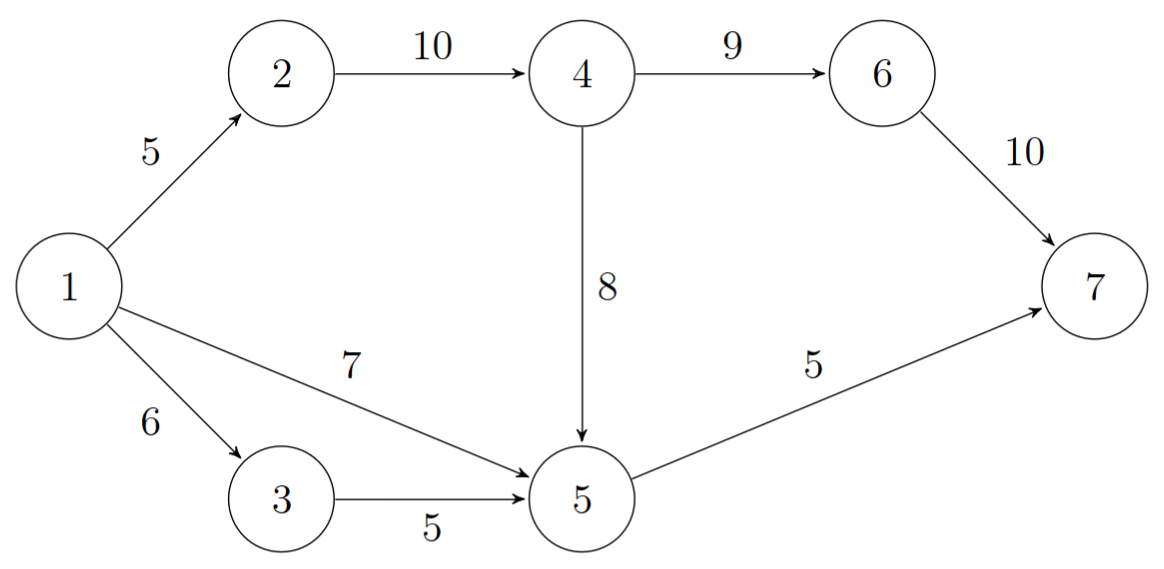
\includegraphics[width=0.3\textwidth]{graph2.png}
    \label{fig:graph2}
\end{figure} 
\noindent

\subsubsection{Finde Eulerpfad bzw. Eulerkreis}
\textit{Nehmen Sie an, die Kanten seien ungerichtet und ungewichtet. Gibt es einen Eulerpfad\index{Eulerpfad} bzw. einen Eulerkreis\index{Eulerkreis}? Warum/Warum nicht? Falls ja, geben Sie diesen an!} \cite{hauptklausur21} \newline 

\subsubsection{Ergebnis von Kruskal}
\textit{Nehmen Sie nun an, der Graph sei ungerichtet und gewichtet. Was ist das Ergebnis des Algorithmus von Kruskal\index{Kruskal}, wenn dieser nach der 5-ten Iteration gestoppt wird? Geben Sie die gefundenen Kanten zu diesem Zeitpunkt an, in der Reihenfolge, wie sie vom Algorithmus ausgewählt werden!} \cite{hauptklausur21}\newline

\subsubsection{Kürzeste Pfade Baum}
\textit{Nehmen Sie an, dass die Kanten gerichtet und gewichtet sind. Wie sieht der durch den \index{Dijkstra}Dijkstra-Algorithmus gefundene kürzeste Pfadebaum mit Start in 1 aus, wenn der Algorithmus nach 5 Iterationsschritten der äußersten Schleife gestoppt wird. Geben Sie den kürzeste Pfadebaum, wie in der Vorlesung, durch die beiden Arrays pred (Vorgänger) und pi (kürzeste Wege) an.} \cite{hauptklausur21} \newline 

\subsubsection{Der Graph als Flussnetzwerk}
\textit{Nehmen Sie an, der Graph sei ein Flussnetzwerk\index{Flussnetzwerk} mit Source 1 und Target 7 mit gerichteten Kanten. Geben Sie einen maximalen Fluss für diesen Graphen an, welcher mit dem Edmond-Karp Algorithmus\index{Edmond-Karp Algorithmus} gefunden werden kann.Zeigen Sie mit einem aus der Vorlesung bekannten Verfahren, dass dieser Fluss\index{Fluss!maximaler} maximal ist.} \cite{hauptklausur21}

\newpage
\section{Linear Programming}
\newpage
\subsection{Verwandeln Sie folgendes LP in ein LP in Standardform}
\begin{action}[title=Ein LP in Standardform bringen] \index{Standardform}
Ein LP in Standartform hat folgende eigenschaften: 
\begin{itemize}
    \item nur nicht-negative Variablen
    \item Gleichungen anstatt Ungleichungen
\end{itemize}
Also müssen die Ungleichungen in Gleichungen umgewandelt werden, negative Variablen in positive umgewandelt werden und anschließend wird das die Zielfunktion\index{Zielfunktion} umformuliert. 
\end{action}
a.
\begin{figure} [H]
    \centering
    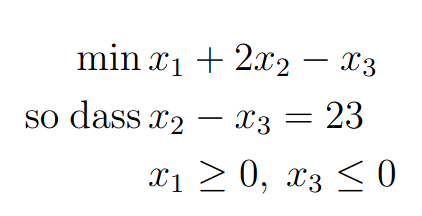
\includegraphics[width=0.3\textwidth]{LPa.png}
    \caption{\cite{probeklausur24}}
    \label{fig:LPa}
\end{figure} 
\noindent
b.
\begin{figure} [H]
    \centering
    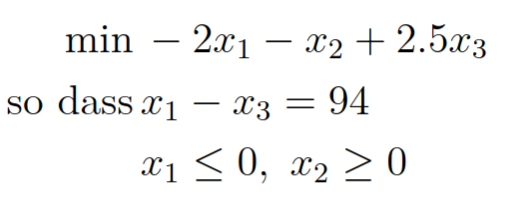
\includegraphics[width=0.3\textwidth]{lpb.png}
    \label{fig:lpb}
    \caption{\cite{hauptklausur21}}
\end{figure} 
\noindent
c.  \cite{probeklausur21} 
\large
\begin{align*}
\text{min} \quad & 2x_1 + 2x_2 \\
\text{so dass} \quad & x_1 + x_2 \leq 42 \\
                      & x_1 \leq 0
\end{align*}
\normalsize
\newline
\begin{minipage}{8cm}
\begin{definitionbox}[title=Schlupfvariablen]
\index{Schlupfvariable} Schlupfvariablen sind spezielle Variablen, die eingeführt werden, um Ungleichungen in Gleichungen zu verwandeln. \newline \newline
Zum Beispiel: Wenn eine Nebenbedingung\index{Nebenbedingungen} 
\[
x_1+2x_2 \leq 4
\]
lautet, wird eine Schlupfvariable\index{Schlupfvariable} $s_1 \geq 0$ hinzugefügt, um dies in eine Gleichung zu verwandeln:
\[
x_1+2x_2+s_1=4
\]
\end{definitionbox}
\end{minipage}
\bigskip
\begin{minipage}{0.2cm}
$\ $
\end{minipage}
\begin{minipage}{9.8cm}
\textbf{Negative Variablen in positive und Ungleichungen in Gleichungen umwandeln m.H. von Schlupfvariablen\index{Schlupfvariable}}
\begin{align*}
    &  x_1 \leq 0 \\
    \text{wird zu} \quad  & x_1 = -z_2  \\
    \text{mit} \quad  & z_2 \geq 0  
\end{align*}
und 
\begin{align*}
    & x_1 + x_2 \leq 42 \\
    \text{wird zu} \quad  & x_1 + x_2 + z_1 = 42 \\
    \text{mit} \quad & z_1 \geq 0 
\end{align*}
\end{minipage}

Daraus kann man direkt formen: 
\begin{align*}
    & -z_2 + x_2 + z_1 = 42 \\
    \text{mit} \quad & x_2, z_1, z_2 \geq 0 \\
\end{align*}

\textbf{Zielfunktion umformulieren}\index{Zielfunktion}
\begin{align*}
    \text{aus} \quad & \text{minimiere} \quad  2x_1 + 2x_2 \\
    \text{wird} \quad & \text{minimiere} \quad  2(-z_2) + 2x_2 \\
    \text{bzw.} \quad & \text{minimiere} \quad  -2z_2 + 2x_2 \\
\end{align*}
\textbf{Daraus entsteht:}
\begin{align*}
    \text{minimiere} \quad &   2x_1 + 2x_2 \\
    \text{so dass} \quad & -z_2 + x_2 + z_1 =    42 \\
    \text{mit} \quad & x_2, z_1, z_2 \geq 0 \\
\end{align*}
\noindent
\begin{minipage}{7cm}
\begin{definitionbox}[title=Basisvariablen]
Basisvariablen\index{Basisvariablen} sind die Variablen, die in einer Basislösung\index{Basislösung} eines linearen Programms\index{LP} nicht auf Null gesetzt werden. \newline
Um sie zu finden, muss die Gleichung zuerst in Standard- oder Schlupfform gebracht werden. \newline
In der Ausgangsform des Simplex-Verfahrens wählt man typischerweise die Schlupfvariablen als Basisvariablen. \newline 

\end{definitionbox}
\end{minipage}
\begin{minipage}{0.5cm}
$\ $
\end{minipage}
\begin{minipage}{10.5cm}
\begin{action}[title=Umwandlung in Schlupfform]\index{Schlupfform}
\begin{minipage}{4cm} 
\textbf{Prinzip:}
\[
\mathbf{\textcolor{BlueViolet}{x_1}} + 
\mathbf{\textcolor{Magenta}{x_2}} \leq
\mathbf{\textcolor{OliveGreen}{n}}
\]
wird zu
\[
\mathbf{\textcolor{Sepia}{x_3}} = \mathbf{\textcolor{OliveGreen}{n}} - 
\mathbf{\textcolor{BlueViolet}{x_1}} - 
\mathbf{\textcolor{Magenta}{x_2}} 
\]
\end{minipage}
\begin{minipage}{0.5cm}
$\ $
\end{minipage}
\begin{minipage}{4cm}
\textbf{Beispiel:} \cite{folien5}
\[
\mathbf{\textcolor{BlueViolet}{15x_1}} + 
\mathbf{\textcolor{Magenta}{5x_2}} \leq
\mathbf{\textcolor{OliveGreen}{480}}
\]
wird zu
\[
\mathbf{\textcolor{Sepia}{x_3}} = \mathbf{\textcolor{OliveGreen}{480}} - 
\mathbf{\textcolor{BlueViolet}{15x_1}} - 
\mathbf{\textcolor{Magenta}{5x_2}} 
\]
\end{minipage}
\end{action}
\end{minipage} 

\vspace{1cm} \noindent
In einem linearen Programm hat eine Basislösung in jeder Zeile des Gleichungssystems genau eine Basisvariable. Dies ist eine direkte Folge der mathematischen Struktur des Simplex-Verfahrens und der Definition von Basisvariablen.\newline
Das \textbf{muss} so sein, damit man eine eindeutige Basislösung hat. \newline 

\newpage
\subsection{Gegeben sei folgendes LP \index{LP} in Schlupf-Form \index{Schlupf-Form}. Was ist die Basislösung\index{Basislösung}? Ist diese zulässig? Warum/Warum nicht?} \newline    



\begin{minipage}{10cm}
\begin{action}[title=Bestimmung der Basislösung\index{Basislösung} eines LP\index{LP}s und deren Zulässigkeit]
Um eine Basislösung\index{Basislösung} zu bestimmen, setzt man zuerst die Nicht-Basisvariablen\index{Basisvariablen!Nicht-} (frei wählbare Variablen) auf 0 und berechnet dann die Werte der abhängigen Variablen. \newline
Eine Basislösung\index{Basislösung} ist zulässig, wenn alle Variablen nicht negativ sind. \newline
Eine Basislösung ist optimal, wenn sie den höchsten möglichen Wert der Zielfunktion\index{Zielfunktion} erreicht.
\end{action}
\end{minipage}
\begin{minipage}{0.5cm}
$\ $
\end{minipage}
\begin{minipage}{7cm}
\begin{definitionbox}[title=Basislösung]
Man muss sowohl die Werte der Basisvariablen\index{Basisvariable}, als auch den Wert der Zielfunktion\index{Zielfunktion} z berechnen! \newline
Ansonsten ist die Basislösung\index{Basislösung} nicht vollständig. 
\end{definitionbox}
\end{minipage}

\bigskip \noindent
a.
\begin{figure} [H]
    \centering
    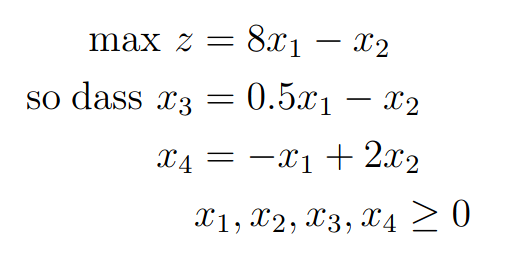
\includegraphics[width=0.3\textwidth]{schlupfa.png}
    \label{fig:schlupfa}
    \caption{\cite{probeklausur24}}
\end{figure} 

\noindent
b.
\begin{figure} [H]
    \centering
    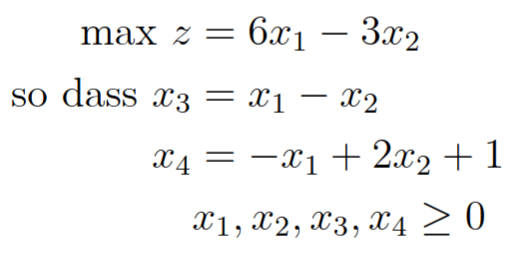
\includegraphics[width=0.3\textwidth]{schlupfb.png}
    \label{fig:schlupfb}
    \caption{\cite{hauptklausur21}}
\end{figure} 

\noindent
c. \newline \normalsize
\textit{Was ist die Basislösung\index{Basislösung} in folgendem LP\index{LP}? Ist diese Basislösung \index{Basislösung} zulässig? Welchen Wert hat die Zielfunktion für die Basislösung? Ist die Basislösung \index{Basislösung} optimal? Warum / warum nicht?} \cite{probeklausur21}
\begin{align*}
    \text{maximiere} \quad & z = x_1 - x_2 \\
    \text{so dass} \quad & x_3 = x_1 + x_2 + 3 \\
                          & x_4 = 2x_1 - x_2 + 2 \\
                          & x_1, x_2, x_3, x_4 \geq 0
\end{align*}
\textbf{Basislösung} \newline
\begin{align*}
    & x_3 = 0 + 0 + 3 = 3\\
   &  x_4 = 2*0 - 0 + 2 = 2\\
\end{align*}
\[
(x_1,x_2,x_3,x_4)=(0,0,3,2)
\]
\textbf{Zulässigkeit} \newline
Alle Variablen sind Positiv, daher ist die Basislösung\index{Basislösung} zulässig.  \newline \newline
\textbf{Wert für die Zielfunktion und Optimalität} 
\[
z = x_1 + x_2 = 0 - 0 = 0
\]
Würde man ein größeres $x_1$ wählen, so wäre auch der Wert der Zielfunktion\index{Zielfunktion} größer. Daher ist die Lösung nicht optimal.

\newpage
\begin{vsbox}[title=Standardform vs. Schlupfform] \index{Schlupfform} \index{Standardform}
\begin{minipage}{8cm} 
\textbf{Formale Definition der Standardform\index{Standardform}: }
\begin{align*}
    \text{max} \quad & \sum_{\textcolor{Maroon}{j=1}}^{\textcolor{Maroon}{n}} c_j x_j \\
    \text{so dass} \quad & \sum_{\textcolor{Maroon}{j=1}}^{\textcolor{Maroon}{n}} a_{ij} x_j \leq b_i \quad \text{für alle } 1 \leq i \leq m \\
    & x_j \geq 0 \quad \text{für alle } 1 \leq j \leq n \\
\end{align*}
\end{minipage}
\begin{minipage}{0.5cm}
$\ $
\end{minipage}
\begin{minipage}{8cm}
\textbf{Formale Definition der Schlupfform:\index{Schlupfform}}
\begin{align*}
    \text{max} \quad & z = \textcolor{Maroon}{\nu} + \sum_{\textcolor{Maroon}{j \in N}} c_j x_j \\
    \text{so dass} \quad & x_i = b_i - \sum_{\textcolor{Maroon}{j \in N}} a_{ij} x_j \quad \text{für } i \in B\\
    & x_i \geq 0 \quad \text{für } i \in B \cup N \\
\end{align*}
\end{minipage}
% Bruch 
\begin{minipage}{8cm}
\begin{itemize}
    \item Ungleichungen \textbf{nicht erlaubt}
    \item Variablen \textbf{nicht negativ} 
    \item die Nicht-Basisvariablen\index{Basisvariablen!Nicht-} und Basisvariablen\index{Basisvariablen} stehen \textbf{"frei"} in den Gleichungen herum
\end{itemize}
\end{minipage}
\begin{minipage}{0.5cm}
$\ $
\end{minipage}
\begin{minipage}{8cm}
\begin{itemize}
    \item Ungleichungen \textbf{nicht erlaubt}
    \item Variablen \textbf{nicht negativ} 
    \item Basisvariablen \index{Basisvariablen} \textbf{in Abhängigkeit} von Nicht-Basisvariablen\index{Basisvariablen!Nicht-} dargestellt
\end{itemize}
\end{minipage}
% Bruch 
\begin{minipage}{8cm}
\bigskip \textbf{Beispiel:}
\begin{align*}
        \text{max} \quad &  z = 3x_1 + 2x_2 \\
    \text{so dass} \quad & x_1+2x_2+s_1 = 4 \\
    & 3x_1+2x_2-s_2=6  \\
    \text{und}\quad & x_1,x_2,s_1,s_2 \geq 0 \\
\end{align*}
\end{minipage}
\begin{minipage}{0.5cm}
$\ $
\end{minipage}
\begin{minipage}{8cm}
\bigskip \textbf{Beispiel:}
\begin{align*}
    \text{max} \quad &  z = 3x_1 + 2x_2 \\
    \text{so dass} \quad & s_1=4-x_1-2x_2 \\
    & s_2=3x_1+2x_2-6 \\
    \text{und}\quad &  x_1,x_2,s_1,s_2 \geq 0 \\
\end{align*}
\end{minipage} 

\end{vsbox}

\newpage
\subsection{Simplex-Verfahren}
\begin{algorithm}[H]
\caption{Simplex-Verfahren}\label{alg:weighted_vertex_cover}
    \centering
    \begin{tabular}{p{10cm} p{7cm}}
        finde Initiallösungen & \\
        \textbf{while} Lösung ist nicht optimal \textbf{do} & \\
        \setlength\parindent{12pt} Pivotschritt zu einem vielversprechenden nächsten Extremwert & \\
        \textbf{end while} & \\
    \end{tabular}
    \label{tab:my_label}
\end{algorithm}


\subsubsection{Führen Sie in folgendem \index{LP} LP einen Pivotschritt\index{Pivotschritt} durch:}
\begin{definitionbox}[title=Entering und Leaving Variables]

\end{definitionbox}
\textbf{Beispielrechnung} \newline
\begin{align*}
\text{max} \quad z &= 23x_1 + 13x_2 \\
\text{mit} \quad x_3 &= 480 - 15x_1 - 5x_2 \\
x_4 &= 160 - 4x_1 - 4x_2 \\
x_5 &= 1190 - 20x_1 - 35x_2 \\
& x_1, x_2, x_3, x_4, x_5  \geq 0
\end{align*}
Die Entering-Variable\index{Entering-Variable} könnte $x_1$ oder $x_2$ sein, da: 
\[
z = 23\textcolor{Peach}{x_1} + 13\textcolor{Peach}{x_2 }
\]
Beide würden die Lösung verbessern. Wir wählen einfach mal $x_1$.\newline
Jetzt müssen wir berechnen was der Wert (die Ratio) von dem \textcolor{RedViolet}{Koeffizienten} der Entering-Variable durch das jeweilige "\textcolor{BlueViolet}{b}" der Gleichung ist. 
\begin{align*}
\text{max} \quad z &= 23x_1 + 13x_2 \\
\text{mit} \quad x_3 &= \textcolor{BlueViolet}{480} - \textcolor{RedViolet}{15}x_1 - 5x_2 \\
x_4 &= \textcolor{BlueViolet}{160} - \textcolor{RedViolet}{4}x_1 - 4x_2 \\
x_5 &= \textcolor{BlueViolet}{1190} - \textcolor{RedViolet}{20}x_1 - 35x_2 \\
& x_1, x_2, x_3, x_4, x_5  \geq 0
\end{align*}
Die Ratios ergeben:
\begin{align*}
    \frac{\textcolor{BlueViolet}{480}}{\textcolor{RedViolet}{15}} & = 32 & \text{ für } x_3\\
    \frac{\textcolor{BlueViolet}{160}}{\textcolor{RedViolet}{4}} & = 40 & \text{ für } x_4 \\
    \frac{\textcolor{BlueViolet}{1190}}{\textcolor{RedViolet}{20}} & = 59.2 & \text{ für } x_5 \\
\end{align*}
Die Leaving-Variable\index{Leaving-Variable} wird die mit der kleinsten Ratio, also $x_3$. \newline
Nun formen wir die zur Leaving-Variable\index{Leaving-Variable} ($x_3$) gehörende Gleichung  nach der Entering-Variable\index{Entering-Variable} ($x_1$) um. 
\begin{align*}
    x_3 &= 480 - 15x_1 - 5x_2 \\
    x_3 + 15x_1 & = 480 - 5x_2 \\
    15x_1 & = 480 - 5x_2 - x_3 \\
    \frac{15}{15}x_1 & = \frac{480}{15} - \frac{5}{15}x_2 - \frac{1}{15}x_3 \\
    x_1 & = 32 - \frac{1}{3}x_2 - \frac{1}{15}x_3 \\
\end{align*}
\noindent
Nun müssen wir noch das LP\index{LP} updaten mit der neuen Variable: 
\begin{align*}
    z  &= 23(32 - \frac{1}{3}x_2 - \frac{1}{15}x_3) + 13x_2 \\
    &= 736 - \frac{23}{3}x_2  - \frac{23}{15}x_3 + 13x_2 \\ 
&= 736  - \frac{23}{15}x_3 + \frac{16}{3}x_2 \\
\end{align*}
\begin{align*}
    x_1 & = 32 - \frac{1}{3}x_2 - \frac{1}{15}x_3  \\
\end{align*}
\begin{align*}
x_4 
&= 160 - 4(32 - \frac{1}{3}x_2 - \frac{1}{15}x_3) - 4x_2  \\
&= 160 - 128 + \frac{4}{3}x_2 + \frac{4}{15}x_3 - 4x_2 \\
&=  32  + \frac{4}{15}x_3 - \frac{8}{3}x_2 \\
\end{align*}
\begin{align*}
    x_5 &= 1190 - 20(32 - \frac{1}{3}x_2 - \frac{1}{15}x_3) - 35x_2 \\
    &= 1190 - 640 + \frac{20}{3}x_2 + \frac{20}{15}x_3 - 35x_2 \\
    &= 550 + \frac{20}{3}x_2 + \frac{20}{15}x_3 - \frac{105}{3}x_2 \\
     &= 550  + \frac{20}{15}x_3 - \frac{85}{3}x_2 \\
     &= 550  + \frac{4}{3}x_3 - \frac{85}{3}x_2 \\
\end{align*}
Das LP\index{LP} sieht nach dem Pivotschritt\index{Pivotschritt} also folgendermaßen aus: 
\begin{align*}
\text{max} \quad z &= 736  - \frac{23}{15}x_3 + \frac{16}{3}x_2 \\
\text{mit} \quad x_1 & = 32 - \frac{1}{3}x_2 - \frac{1}{15}x_3  \\
x_4 &=  32  + \frac{4}{15}x_3 - \frac{8}{3}x_2 \\
x_5  &= 550  + \frac{4}{3}x_3 - \frac{85}{3}x_2 \\
\end{align*}
\hline
a.
\begin{figure} [H] 
    \centering
    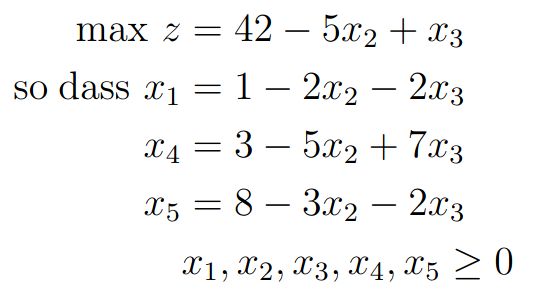
\includegraphics[width=0.3\textwidth]{pivota.png}
    \caption{\cite{probeklausur24}}
    \label{fig:pivota}
\end{figure} 
 
b.
\begin{figure} [H]
    \centering
    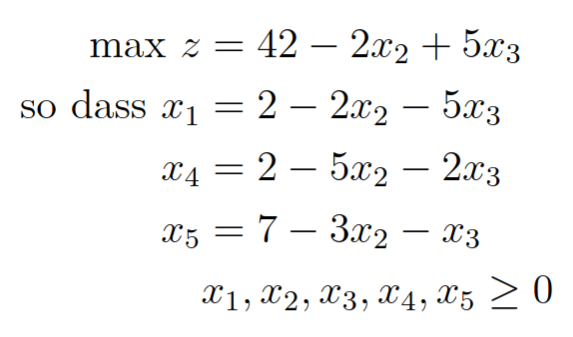
\includegraphics[width=0.3\textwidth]{pivotb.png}
    \caption{\cite{hauptklausur21}}
    \label{fig:pivotb}
\end{figure} 

c.\cite{probeklausur21}
\begin{align*}
    \text{maximiere} \quad & z = 2x_1 - 3x_2 \\
    \text{so dass} \quad & x_3 = 2 - x_1 + x_2 \\
                          & x_4 = 3 + 2x_1 - 2x_2 \\
                          & x_1, x_2, x_3, x_4 \geq 0
\end{align*}

Die Eingangsvariable könnten $x_1$ oder $x_2$ sein, da: 
\[
z = 2\textcolor{Peach}{x_1} + 3\textcolor{Peach}{x_2 }
\]
Wir wählen $x_1$ als Entering-Variable\index{Entering-Variable}. \newline
Jetzt müssen wir berechnen was der Wert (die Ratio) von dem \textcolor{RedViolet}{Koeffizienten}\index{Pivotkoeffizient} der Entering-Variable durch das jeweilige "\textcolor{BlueViolet}{b}" der Gleichung ist. 
\begin{align*}
 x_3 &= \textcolor{BlueViolet}{2} - \textcolor{RedViolet}{1}x_1 + x_2 \\
x_4 & = \textcolor{BlueViolet}{3} + \textcolor{RedViolet}{2}x_1 - 2x_2 \\
\end{align*}
Die Ratios sind: 
\begin{align*}
    \frac{2}{1} &= 0.5 & \quad \text{für } x_3 \\
    \frac{3}{2} & \approx 0.6 & \quad  \text{ für } x_3 \\
\end{align*}
Die Leaving-Variable\index{Leaving-Variable} wird die mit der kleinsten Ratio, also $x_3$. \newline
Nun formen wir die zur Leave-Variable ($x_3$) gehörende Gleichung nach der Entering-Variable ($x_1$) um.
\begin{align*}
    x_3 &= 2 - x_1 + x_2 \\
    x_1 + x_3 &= 2 + x_2 \\
    x_1  &= 2 + x_2  - x_3 \\
\end{align*}
Nun müssen wir noch das LP updaten mit der neuen Variable:
\begin{align*}
    z &= 2x_1 - 3x_2 \\
    &= 2(2 + x_2  - x_3) - 3x_2 \\
    &= 4 + 2x_2  - 2x_3 - 3x_2 \\
    &= 4 - 2x_3  - x_2 \\
\end{align*}
\begin{align*}
     x_4 &= 3 + 2(2 + x_2  - x_3) - 2x_2 \\
     &= 3 + 4 + 2x_2  - 2x_3 - 2x_2 \\
     &= 7 - 2x_3 \\
\end{align*}
Das LP sieht nach dem Pivotschritt\index{Pivotschritt} also folgendermaßen aus:
\begin{align*}
    \text{maximiere} \quad & z = 4 - 2x_3  - x_2 \\
    \text{so dass} \quad & x_1  = 2 + x_2  - x_3 \\
                          & x_4 = 7 - 2x_3 \\
                          & x_1, x_2, x_3, x_4 \geq 0
\end{align*}
\newpage
\subsection{Formen Sie folgendes LPaux\index{LPaux} um, so dass es eine gültige Basislösung\index{Basislösung} hat und geben Sie diese an! }
Besitzt die Grundform\index{Grundform} des LPs eine Lösung? Warum/Warum nicht? Falls Sie es nach einem Pivotschritt\index{Pivotschritt} nicht beurteilen können, geben Sie einen Grund an. \newline

a.
\begin{figure} [h!]
    \centering
    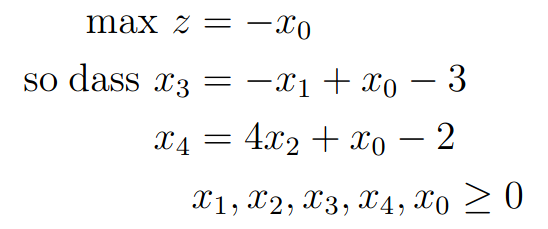
\includegraphics[width=0.3\textwidth]{lpauxa.png}
    \label{fig:lpauxa}
    \caption{\cite{probeklausur24}}
\end{figure} 
\newline
b.
\begin{figure} [h!]
    \centering
    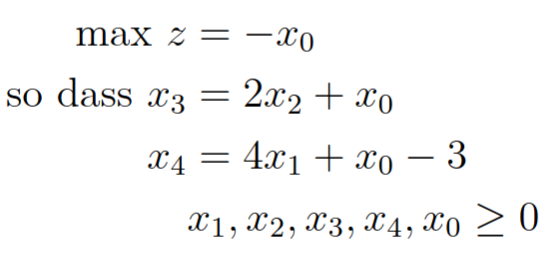
\includegraphics[width=0.3\textwidth]{lpauxb.png}
    \label{fig:lpauxb}
    \caption{\cite{hauptklausur21}}
\end{figure} 
\newpage
\subsection{Besitzt folgendes LP \index{LP} eine zulässige Lösung? Warum / warum nicht?} 
a.
\begin{figure} [h!]
    \centering
    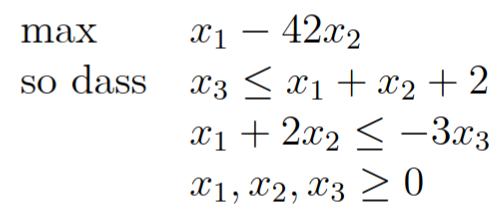
\includegraphics[width=0.3\textwidth]{zulaessigc.png}
    \caption{\cite{probeklausur21}}
    \label{fig:zulaessigc}
\end{figure} 

\newpage
\section{Multiple Choice}
\begin{longtable}[H]
    \centering
    \begin{tabular}{ | p{1cm} | c c | p{13cm} |} \hline
    & & & \\
     & \textbf{Richtig} & \textbf{Falsch} &  \\ & & & \\ \hline \hline  & & & \\
     \cite{probeklausur21}\cite{hauptklausur21}\cite{probeklausur24} & $\square$ &  \checkedbox  &  In einem Flussnetzwerk\index{Flussnetzwerk} ist für einen gültigen Fluss\index{Fluss} die Kapazität jedes Schnittes\index{Cut} (Cuts) gleich.\\ & & & \\  \hline \hline & & & \\
     \cite{probeklausur21}\cite{probeklausur24} & $\square$ &  \checkedbox & Der Simplex-Algorithmus\index{implex-Algorithmus} kann mit vier möglichen Ausgängen enden: Optimale Lösung\index{Lösung!optimale}, LP ungültig, LP\index{LP} unbeschränkt oder lokales, aber nicht globales Optimum des LPs. \\ & & & \\
     \cite{nachklausur19} & \checkedbox &  $\square$   & Wenn die Basislösung\index{Basislösung} des LP ungültig ist, besitzt das LP keine zulässige Lösung. \\ & & & \\ \hline \hline & & & \\
     
     \cite{probeklausur21}\cite{probeklausur24} & $\square$ &  \checkedbox  & Das folgende Problem ist NP-hart\index{NP-hart}: Gegeben sei ein gerichteter, gewichteter Graph. Gibt es einen negativen Kreis? \\ & & & \\
     
     \cite{nachklausur19} & \checkedbox &  $\square$  & Das Problem, gegeben eine beliebige nichtlineare Funktion\index{Funktion!nichtlineare}, finde ein globales Optimum,\index{Optimum!globales} ist NP schwer\index{NP schwer}.\\ & & & \\
     
     & & & Das folgende Problem ist in polynomieller Laufzeit\index{Laufzeit!polynomielle} lösbar:\\ & & & \\
     
     \cite{nachklausur19} & $\square$ &  \checkedbox  &  Gegeben lineare Ungleichungen der Form $w_1^ix_1+...+w_n^i x_n \leq b^i$ , entscheide, ob es eine Lösung gibt, die maximal vier Ungleichungen nicht erfüllt. \\ & & & \\
     
     \cite{nachklausur19}& $\square$ & \checkedbox  & Gegeben eine aussagenlogische Formel in konjunktiver Normalform\index{Normalform!konjunktive}, finde eine Belegung der Variablen, so dass maximal viele Klauseln erfüllt sind.  \\& & & \\
     
     \cite{probeklausur21}\cite{probeklausur24} & \checkedbox &  $\square$  &  Gegeben eine Anzahl von Räumen und Veranstaltungen, die in gewissen Räumen stattfinden können. Existiert eine Zuordnung aller Veranstaltungen zu Räumen, so dass kein Raum doppelt belegt ist? \\ & & & \\\hline \hline & & & \\  
     
     \cite{probeklausur21}\cite{probeklausur24} & $\square$ &  \checkedbox  &  Das Problem einen minimalen Fluss\index{Fluss!minimaler} in einem Flussgraphen\index{Flussgraph} (V, (E, c)) zu finden, kann man als\index{LP} LP mit |E| Variablen und 3 · |V| Nebenbedingungen\index{Nebenbedingungen} schreiben. \\ & & & \\\hline \hline & & & \\
     
     & & & Bei einem gerichteten Graphen mit nicht-negativen Kantengewichten ist der kürzesten Pfad zwischen 2 Knoten eindeutig, wenn ... \\ & & & \\
     
     \cite{probeklausur24}\cite{hauptklausur21} & $\square$ & \checkedbox &  ...alle Kantengewichte unterschiedliche Potenzen von 2 sind. \\ & & & \\
     \cite{probeklausur24}& $\square$ &  \checkedbox & ...alle Kantengewichte unterschiedliche positive ganze Zahlen sind
und der Graph keine Zyklen enthält. \\ & & & \\

    \cite{hauptklausur21}& \checkedbox &  $\square$  & ...alle Kantengewichte unterschiedliche, positive ganze Zahlen sind. \\ & & & \\ \hline \hline & & & \\ 
    
    \end{tabular}
    \label{tab:mutiple_choice}
\end{longtable}


\begin{table}[]
    \centering
    \begin{tabular}{ | p{1cm} | c c | p{13cm} |} \hline
    & & & \\
     & \textbf{Richtig} & \textbf{Falsch} &  \\ & & & \\ \hline \hline  & & & \\
         & & &  Wir betrachten einen gerichteten Graphen und einen Startknoten. Wir nehmen an, dass einige Kantengewichte negativ sind, es aber keine Zyklen in dem Graphen gibt. Wenn wir den\index{Dijkstra} Dijkstra-Algorithmus anwenden... \\ & & & \\
         
     \cite{probeklausur24}\cite{probeklausur21} & $\square$ &  \checkedbox & ...könnte der Algorithmus in eine Endlosschleife geraten. \\ & & & \\
     
     \cite{probeklausur24}& \checkedbox &  $\square$  & ...wird der Algorithmus garantiert terminieren, aber in einigen Fällen kann es passieren, dass die kürzesten Pfade nicht alle korrekt sind. \\ & & & \\
     
     \cite{probeklausur21} & \checkedbox &  $\square$  & Die Greedy Idee, welche der Dijkstra\index{Dijkstra} Algorithmus anwendet, kann nicht auf einem Graphen mit negativen Kantengewichten angewendet werden! \\ & & & \\
      
     \cite{probeklausur24} \cite{probeklausur21} & $\square$ &  \checkedbox  & ...wird der Algorithmus garantiert terminieren und in einigen Fällen sind tatsächlich die kürzesten Pfade alle korrekt.\\ & & & \\ \hline \hline & & & \\
     
     \cite{hauptklausur21} & $\square$ &  \checkedbox  & Die Komplexität des Problems alle kürzesten Pfade\index{Pfad!kürzeste} in einem Graphen mit negativen Kantengewicht\index{Kantengewicht!negatives} zu finden ist immer in $\Omega(|V|^3)$. \\ & & & \\ \hline \hline & & & \\ 
     
     \cite{hauptklausur21} & \checkedbox * &  $\square$  &  Gegeben sei ein gerichteter und gewichteter Graph G = (V, E, W ). Die Länge des längsten Pfades zwischen 2 beliebigen Knoten zu finden, wenn der Graph azyklisch ist, kann in $O(|V|^3)$ gelöst werden. \\ & & & \\
     
     \cite{hauptklausur21}  & \checkedbox * &  $\square$  &  Gegeben sei ein gerichteter und gewichteter Graph G = (V, E, W ). Die Länge des längsten, azyklischen Pfades\index{Pfad!azyklischer} zwischen 2 beliebigen Knoten zu finden, wenn alle Kantengewichte nicht negativ sind, kann in $O(|V|^3)$ gelöst werden. \\ & & & \\
     
      \cite{hauptklausur21}  & \checkedbox * &  $\square$  & Gegeben sei ein gerichteter und gewichteter Graph G = (V, E, W ). Die Länge des längsten, azyklischen Pfades\index{Pfad!azyklischer} zwischen 2 beliebigen Knoten zu finden, kann in $O(|V|^3)$ gelöst werden.  \\ & & & \\
       % & $\square$ &  $\square$  & \\ & & & \\ %
        %& $\square$ &  $\square$  & \\ & & & % 
        & & & *\textit{Es kann deutlich effizienter gelöst werden, aber die effizientere Lösung würde genau genommen immer noch in $O(|V|^3)$ liegen!} \\ & & & \\
        \hline \hline & & & \\
        
    \cite{nachklausur19}    & \checkedbox &  $\square$  & Der minimale Produktspannbaum\index{Spannbaum!Produkt-} lässt sich mit dem Prim Algorithmus\index{Prim} berechnen. \\ & & & \\ \hline
    \end{tabular}
    \caption{Caption}
    \label{tab:my_label}
\end{table}


Müssen noch Fragen vom Spickzettel einfügen und Laufzeiten und wie man die Algorithmen anwendet. Algorithmen mit Problemen zusammenführen. 



\addcontentsline{toc}{section}{Index}
\printindex
\addcontentsline{toc}{section}{List of Algorithms}
\listofalgorithms

\addcontentsline{toc}{section}{References}
\printbibliography


\end{document}

